\section{Appendix 1: Theorie gewöhnlicher Differentialgleichungen}
\label{subsec:ode}
\begin{definition}{Gewöhnliche Differentialgleichung}{ode}
Sei $F: \R^n \times \cdots \times \R^n \times \R \to \R^n$ und $x: (a,b) \to \R^n$. Dann ist eine \textbf{gewöhnliche Differentialgleichung (ODE)} $k$\textbf{-ter Ordnung} gegeben durch
\begin{equation}
\frac{d^k x}{dt^k} (t)=F(x(t), x'(t), \dots, x^{(k-1)}(t), t).
\end{equation}
\end{definition}
\begin{definition}{Anfangswertproblem}{awp}
Ein \textbf{Anfangswertproblem (AWP)} für eine ODE in $x: (a,b) \to \R^n$ ist gegeben durch $t_0 \in (a,b)$ mit 
\begin{equation}
x(t_0) = a_0, \ x'(t_0)=a_1, \ \dots, x^{(k-1)}(t_0)=a_{k-1}
\end{equation}
für vorgegebene Konstanten $a_0, \dots, a_{k-1} \in \R^n, t_0 \in \R$.
\end{definition}
\begin{beispiel}
Betrachte $\ddot{x} = -x$. Die Fundamentallösungen sind gegeben durch $\sin(t)$ und $\cos(t)$. Zu $a_0, a_1 \in \R$ ist $x(t)=a_0 \cos(t) + a_1 \sin(t)$ eine Lösung des AWP mit $t_0=0$.
\end{beispiel}
\begin{satz}{Reduktion zur 1. Ordnung}{ordnung}
Eine DGL $k$-ter Ordnung ist äquivalent zu einem System von DGLn 1. Ordnung im $\R^{k+n}$. Für $y = (y_0, y_1, \dots, y_{k-1})$ mit $y_i \in \R^n$ betrachten wir
\begin{align}
\dot{y_0} &= y_1 \\
\dot{y_1} &= y_2 \\
&\vdots \\
\dot{y_{k-1}} &= F(y_0, \dots, y_{k-1}, t)
\end{align}
mit AW
\begin{align}
y_0(t_0) &= a_0 \\
y_1(t_0) &= a_1 \\
&\vdots \\
y_{k-1}(t_0) &= a_{k-1}.
\end{align}
Dann sind die Lösungen der DGL $k$-ter Ordnung bijektiv zu den Lösungen des obigen Systems 1. Ordnung.
\end{satz}
\begin{bemerkung}Autonomie\\
Eine DGL heißt \textbf{autonom}, falls die rechte Seite $F$ nicht explizit von $t$ abhängt.\\
Eine autonome Gleichung 1. Ordnung hat also die Form $\dot{x}=F(x)$.\\
Fasst man $F: \R^n \to \R^n$ als Vektorfeld auf, so sind die Lösungen $x: (a,b) \to \R^n$ dieser Gleichung gerade die \textit{Integralkurven}, die wir zuvor betrachtet haben.
\end{bemerkung}
\begin{theorem}{Satz von Picard-Lindelöf}{picardlindelöf}
Sei $\Os \sub \R^n \times \R$ offen, $F: \Os \to \R^n$ und $(x_0, t_0) \in \Os$ ein AW. Sei außerdem $a, b > 0$ so, dass $A=\overline{B(x_0,b)} \times [t_0 -a, t_0+a] \sub \Os$ und $F|_A$ \textit{lipschitzstetig} bezüglich $x$ mit der Konstante $K$ ist. Definiere $M:= \max \{||F(x,t)||, (x,t) \in A \}$ und $\alpha := \min \left( a, \frac{b}{M}, \frac{1}{2K}\right)$.\\
Unter diesen Voraussetzungen hat das AWP
\begin{align}
\dot{x}(t) &= F(x, t) \\
x(t_0)=x_0
\end{align}
genau eine Lösung $x: [t_0 - \alpha, t_0 + \alpha] \to \R^n$ mit Bild in $\overline{B(x_0,b)}$.
\begin{figure}[H]
\label{fig:picard}
\centering
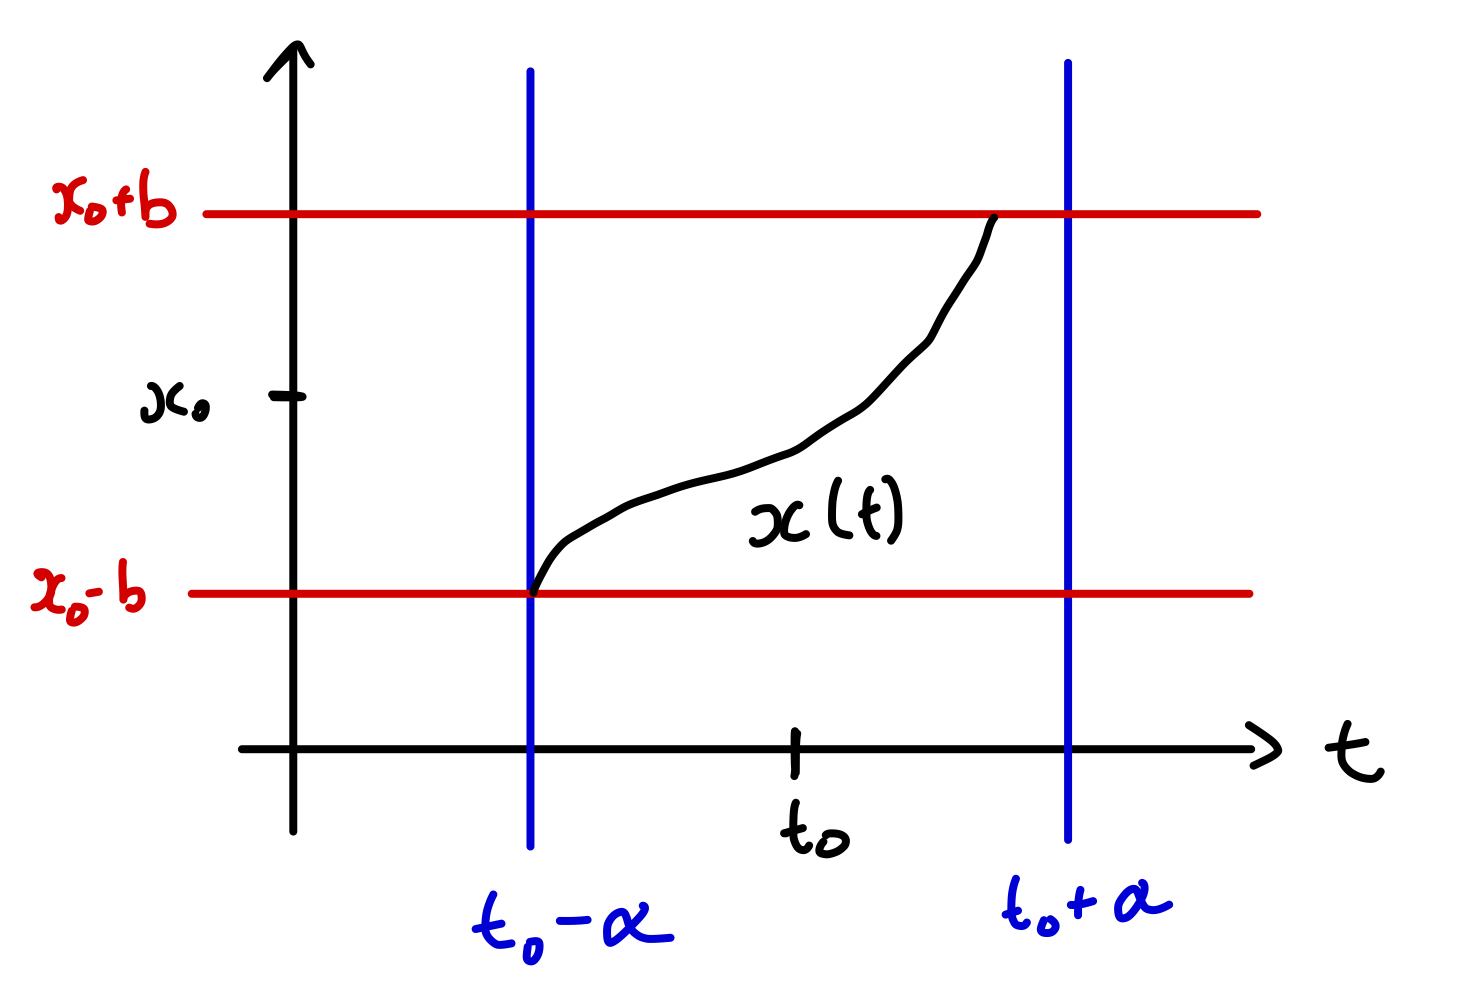
\includegraphics[width=0.3\linewidth]{Bilder/picard.png}
\caption{Auf einer Umgebung von $t_0$ ist das AWP eindeutig lösbar.}
\end{figure}
\end{theorem}
\begin{beweis}
Der Raum $X:= C([t_0 - \alpha, t_0 + \alpha], \overline{B(x_0, b)}$ ist mit der Supremumsnorm ein vollständiger metrischer Raum. Die Menge $Y:= \{ \phi \in X | \phi(t_0)=x_0 \} \sub X$ ist als abgeschlossene Teilmenge auch vollständig.\\
Wir definieren 
\begin{align}
A: Y &\to C([t_0 - \alpha, t_0 + \alpha], \R^n)\\
t &\mapsto (A\phi)(t) := x_0 + \int_{t_0}^t F(\phi(s), s) ds.
\end{align}
Nun zeigt man:
\begin{itemize}
\item $\phi \in Y \implies A\phi \in Y$
\item $A: Y \to Y$ ist eine Kontraktion.
\item Der Fixpunkt von $A$ löst das AWP.
\item Jede Lösung des AWP ist ein Fixpunkt von $A$ $\rightarrow$ Lösung ist eindeutig.
\end{itemize}
\end{beweis}
\begin{beispiel}Lipschitzbedingung\\
Die Lipschitz-Bedingung ist wesentlich für die Eindeutigkeit der Lösung. Betrachte z.B. $\dot{x} = \sqrt{x}$ auf $\R$. Die rechte Seite ist in $x_0 = 0$ stetig, aber nicht lokal lipschitzstetig. Tatsächlich gibt es zwei Lösungen mit $x(0)=0$: $x(t)\equiv 0$ und $x(t)=\frac{t^2}{4}$.
\end{beispiel}
\begin{satz}{Stetige Abhängigkeit}{stetigeabh}
Sei $\Os \in \R^n \times \R$ offen und $F: \Os \to \R^n$ lipschitzstetig mit Konstante $K$. Seien $(x_0, t_0) \in \Os$ und $(x_0^\ast, t_0) \in \Os$ zwei AW mit lokalen Lösungen 
\begin{align}
\phi: [t_0 - \alpha, t_0 + \alpha] &\to \R^n, \ \phi(t_0)=x_0 \\
\phi^\ast: [t_0 - \alpha, t_0 + \alpha] &\to \R^n, \ \phi^\ast(t_0)=x_0^\ast
\end{align}
des AWP.\\
Dann gilt
\begin{equation}
|| \phi(t)-\phi^\ast(t)|| \leq ||x_0-x_0^\ast||\exp(K|t-t_0|).
\end{equation}
Insbesondere folgt aus $x_0^\ast \to x_0$ die gleichmäßige Konvergenz $\phi \to \phi^\ast$ in $C([t_0-\alpha, t_0 + \alpha], \R^n)$.
\end{satz}
\begin{bemerkung}
Analog, aber aufwändiger ist zu zeigen:\\
Ist $F$ von Klasse $C^k$ mit Schranke $\tau$ an die $C^k-Norm$, so erhalten wir $C^k-Abschätzungen$ für $||\phi - \phi^\ast||_{C^k}$. Ist insbesondere $F \in \cinf{\Os}{\R^n}$, so hängen die Lösungen glatt vom AW $x_0$ ab.
\end{bemerkung}
\begin{satz}{Rektifizierungssatz}{rektifizierung}
Ist $F: M \to TM$ ein glattes Vektorfeld und $F_p \neq 0$, so existiert eine offene Umgebung $U \sub M$ von $p$ mit lokalen Koordinaten $(x_1, \dots, x_n)$, sodass $F|_U = \frac{\partial}{\partial x_1}$. Die Lösungen (Integralkurven) von $\dot{x} = \frac{\partial}{\partial x_1}$ haben dann die einfache Form
\begin{equation}
x_1(t)=t+x_1(0), \ x_2(t)=x_2(0), \ \dots, \ x_n(t)=x_n(0).
\end{equation}
Dies ist die \textit{Normalform} des Vektorfeldes.
\end{satz}
\begin{korollar}{Aus Picard-Lindelöf}{auspiclöf}
Unter der Lipschitz-Voraussetzung stimmen zwei lokale Lösungen
\begin{align}
\phi_1: (a_1, b_1) &\to \R^n \\
\phi_2: (a_2, b_2) &\to \R^n
\end{align}
des AWP $\dot{\phi}(t)=F(\phi(t), t), \ \phi(t_0)=x_0 \ (\ast)$ auf $(a_1, b_1) \cap (a_2, b_2)$ überein.
\end{korollar}
\begin{bemerkung}Konstruktion der maximalen Lösung\\
Mit Korollar \ref{auspiclöf} kann man die maximale Lösung von $\dot{\phi}(t)=F(\phi(t), t), \ \phi(t_0)=x_0$ konstruieren, indem man aus der Menge
\begin{equation}
\Ms := \{\phi_i: (a_i, b_i) \to \R^n | i \in I \}
\end{equation}
den maximalen Definitionsbereich $I_{x_0}= \bigcup_{i \in I} (a_i, b_i)$ bestimmt und $\phi: I_{x_0} \to \R^n$ durch $\phi(t) = \phi_i(t)$ definiert, wenn $t \in (a_i, b_i)$.
\end{bemerkung}
\begin{satz}{Satz über die maximale Lösung}{maxlsg}
Sei $\Os \sub \R^n \times \R$ und $F: \Os \to \R^n$ lipschitzstetig bezüglich $x$ auf jeder kompakten Teilmenge $A \sub \Os$.\\
Falls die maximale Lösung $\phi_{x_0}:(a(x_0), b(x_0)) \to \R^n$ des AWP $(\ast)$ die Bedingung $b(x_0) < \infty$ erfüllt, so existiert zu jeder kompakten Teilmenge $A \sub \Os$ ein $t_A < b(x_0)$, sodass für alle $t \in (t_A, b(x_0))$ gilt: $(\phi_{x_0}(t), t) \cancel{\in} A$.
\end{satz}
\begin{bemerkung}
Eine analoge Aussage gilt für $a(x_0) > - \infty$.
\end{bemerkung}
\begin{korollar}{Vollständigkeit von Vektorfeldern}{vollstvf}
Ist $X \in \Gamma (TM)$ ein Vektorfeld mit kompaktem Träger, so sind die maximalen Integralkurven von $X$ auf ganz $\R$ definiert.
\end{korollar}
Jetzt wenden wir uns einigen Lösungsmethoden für Differentialgleichungen in $\R$ zu.
\begin{satz}{Trennung der Variablen}{vartrennung}
Sei $F$ so, dass es sich schreiben lässt als $F(x,t) = f(x) \cdot g(t)$ mit $\dot{x}(t) = f(x) \cdot g(t), \ x(t_0) = x_0$. Wir betrachten zwei Fälle:
\begin{enumerate}
\item Fall: $f(x_0)=0$: $x(t)\equiv x_0$ ist eine auf ganz $\R$ definierte Lösung.
\item Fall: $f(x_0)\neq 0$: Ist $f$ stetig, so gilt $f(x) \neq 0$ in einer Umgebung von $x_0$, also gilt
\begin{equation}
\frac{\dot{x}}{f(x)} = g(t).
\end{equation}
Sei $F(y)$ eine Stammfunktion von $\frac{1}{f(y)}$, d.h. $F'(y) = \frac{1}{f(y)}$. Dann gilt 
\begin{equation}
\frac{d}{dt}F(x(t)) = F'(x(t)) \cdot \dot{x}(t) = \frac{\dot{x}(t)}{f(x(t))}= g(t).
\end{equation}
Durch Integration folgt
\begin{equation}
F(x(t)) = F(x(t_0)) + \int_{t_0}^t g(s) ds.
\end{equation}
Ist $F$ lokal invertierbar, können wir daraus $x$ bestimmen.
\end{enumerate}
\end{satz}
\begin{beispiele}
\begin{enumerate}
\item Betrachte $\dot{x} = - \frac{x}{t}$ mit $x(1)=x_0$. Hier ist $f(x) = x$ und $g(t)=- \frac{1}{t}$.\\
Im 1. Fall ist $x_0=0$, also ist $x(t) \equiv 0$ eine auf ganz $(0, \infty)$ definierte Lösung.\\
Im 2. Fall ist $x_0 \neq 0$, also
\begin{equation}
F(x) = \int_{x_0}^x \frac{1}{f(y)} dy = \int_{x_0}^x \frac{1}{y} dy = \ln \left( \frac{x}{x_0} \right).
\end{equation}
Außerdem gilt
\begin{equation}
\int_1^t g(\tau) d \tau = \int_1^t - \frac{1}{\tau} d\tau = - \ln (t).
\end{equation}
Somit erhalten wir
\begin{equation}
\ln \left( \frac{x}{x_0} \right) = - \ln (t) \iff x(t) = \frac{x_0}{t}.
\end{equation}
Für alle $x_0 \in \R$ ist die maximale Lösung auf ganz $(0, \infty)$ definiert.
\item Betrachte $\dot{x} = x^2, \ x(0)=x_0$.\\
Im 1. Fall gilt $x_0=0$, also ist $x(t)=0$ eine auf ganz $\R$ definierte Lösung.\\
Im 2. Fall gilt $x_0 \neq 0$, also 
\begin{equation}
F(x) = \int_{x_0}^x \frac{1}{y} dy = - \left.\frac{1}{y} \right|_{x_0}^x = \frac{1}{x_0}- \frac{1}{x}.
\end{equation}
Integration liefert $\int_0^t g(\tau) d\tau = t$. Gleichsetzen und Auflösen nach $x(t)$ ergibt:
\begin{equation}
x(t) = \frac{x_0}{1-x_0t}.
\end{equation}
Ist $x_0>0$, so ist die maximale Lösung auf $(-\infty, \frac{1}{x_0})$ definiert, für $x_0<0$ hingegen auf $(\frac{1}{x_0}, \infty)$.
\end{enumerate}
\end{beispiele}
\begin{satz}{Variation der Konstanten}{varkonst}
Sei eine ODE der Form $\dot{x} = p(t)x + q(t)$ mit AWP $x(t_0) = x_0$ gegeben. Eine solche ODE heißt \textbf{lineare Differentialgleichung}.\\
Die Lösung funktioniert schrittweise:
\begin{enumerate}
\item Schritt: Man löst das vereinfachte Problem mit $q \equiv 0$, also $\dot{x}=p(t)x$. Durch Trennung der Variablen erhalten wir $\frac{\dot{x}}{x}=p(t)$. Also gilt
\begin{equation}
\ln (x(t)) = \int p(\tau) d\tau + C^\ast \implies x(t) = C \cdot \exp \left( \int p(\tau) d\tau \right)
\end{equation}
mit $C = \exp(C^\ast)$.
\item Schritt: Für das eigentliche Problem machen wir den Ansatz
\begin{align}
x(t) &= C(t) \cdot \exp \left( \int p(\tau) d \tau \right)\\
\implies \dot{x}(t) &= \underbrace{\dot{C}(t) \exp \left( \int p(\tau) d\tau \right)}_{=q(t)} +p(t) \cdot \underbrace{C(t) \exp \left( \int p(\tau) d\tau \right)}_{=p(t)x(t)}.
\end{align}
Also folgt, dass $\dot{C}(t) = q(t) \exp \left( -\int p(\tau) d\tau \right)$.
\end{enumerate}
\end{satz}
\begin{beispiel}
Wir betrachten den einfachsten Fall mit konstanten Koeffizienten, also $\dot{x}=px+q$ mit $p,q \in \R \exc \{0\}$.
\begin{enumerate}
\item Wir lösen $\dot{x} = px$ und erhalten $x(t) = C \exp(pt)$.
\item $\dot{C}=q\exp(-pt) \implies C(t) = - \frac{q}{p} \exp(-pt) + D$. Einsetzen in den Ansatz liefert
\begin{equation}
x(t) = \left( - \frac{p}{q} \exp(-pt) + D\right)\exp(pt) = D \exp(pt) - \frac{q}{p}.
\end{equation}
$D$ bestimmt sich aus dem Anfangswert $x_0 = x(0) = D-\frac{q}{p} \implies D = x_0 + \frac{p}{q}$. Also lautet die Lösung $x(t) = \left( x_0 + \frac{p}{q}\right) \exp (pt) - \frac{q}{p}.$
\end{enumerate}
\end{beispiel}
\begin{bemerkung}Matrixexponential\\
Für $A \in \text{L}(\R^n, \R^n)$ konvergiert die Reihe
\begin{equation}
\exp(A) := \Sum{k,0,\infty} \frac{A^k}{k!}.
\end{equation}
Also ist $\exp(A)$ auch eine lineare Abbildung $\R^n \to \R^n$, die \textbf{Matrixexponential} genannt wird. Sie hat folgende Eigenschaften:
\begin{itemize}
\item $\exp(0) = \id$
\item $AB = BA \implies \exp(A+B)=\exp(A)\exp(B)$
\item $\exp(A)$ ist invertierbar mit $\left( \exp(A)\right)^{-1} = \exp(-A)$.
\item Sei $B$ invertierbar. dann gilt $\exp(BAB^{-1}) = B \exp(A) B^{-1}$.
\item $\det \exp(A) = \exp (\Tr A)$.
\end{itemize}
\end{bemerkung}
\begin{beispiele}
\begin{enumerate}
\item Sei $A$ von Diagonalgestalt $A = \diag \{\lambda_1, \dots, \lambda_n \}$. Dann gilt $A^k = \diag \{\lambda_1^k, \dots, \lambda_n^k \}$, womit das Matrixexponential die Gestalt $\exp(A) = \diag \{ \exp(\lambda_1^k), \dots, \exp(\lambda_n^k) \}$ hat.
\item $A= \mat{0,1}{0,0}$ ist nilpotent, also $A^2=0$. Damit gilt $\exp(A) = \mat{1,1}{0,1}=\id+ A$. Dies kann man verallgemeinern:\\
Sei $A=\mat{\lambda, \mu}{0,\lambda} = \lambda \id + \mu \mat{0,1}{0,0}$. Dann gilt:
\begin{equation}
\exp(A) = \mat{\exp(\lambda), 0}{0, \exp(\lambda)} \mat{1, \mu}{0,1} = \mat{\exp(\lambda), \mu \exp(\lambda)}{0, \exp(\lambda)}.
\end{equation}
\item Weiterhin gilt für $A = \mat{0,-a}{a,0}$, dass $A^2=\mat{-a^2, 0}{0, -a^2}$, $A^3 = \mat{0, a^3}{-a^3, 0}$, usw.\\
ÜA: $exp(A) = \mat{\cos a, -\sin a}{\sin a, \cos a}$
\end{enumerate}
\end{beispiele}
\begin{satz}{Matrixexponential-Lösung eines AWP}{awpexp}
Das AWP
\begin{align}
\dot{x} &= Ax \ \text{für} \ A \in \text{L}(\R^n, \R^n)\\
x(t_0) &= x_0
\end{align}
hat die eindeutige Lösung
\begin{align}
x: \R &\to \R^n \\
t &\mapsto x(t):=\exp((t-t_0)A)x_0.
\end{align}
\end{satz}
\begin{beweis}
Nachrechnen.
\end{beweis}
\begin{bemerkung}
Konkrete Fälle im $\R^2$.\\
Wie betrachten im Folgenden immer die Jordan-Form der Matrizen.
\begin{enumerate}
\item Fall: $A=\diag \{\lambda_1, \lambda_2 \}$ mit $\lambda_1 \leq \lambda_2$ reell.\\
Für $x(0)=x_0$ ist die Lösung des AWPs aus dem Satz gegeben durch 
\begin{equation}
\cvc{x_1(t), x_2(t)} = \cvc{\exp(t\lambda_1)x_1(0), \exp(t \lambda_2)x_2(0)}
\end{equation}
\begin{figure}[H]
\label{fig:fall1}
\centering
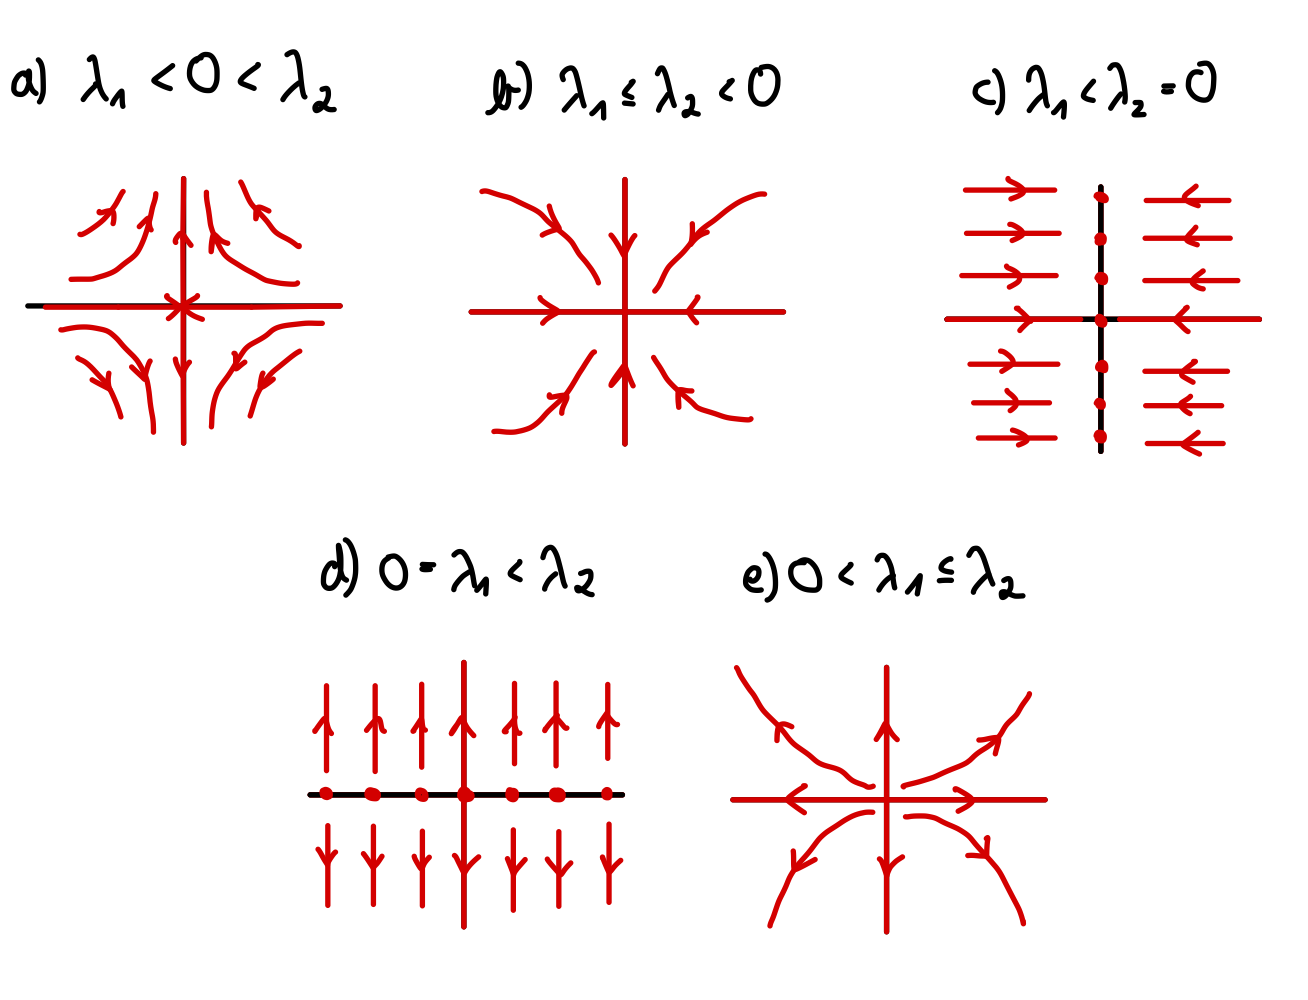
\includegraphics[width=0.5\linewidth]{Bilder/fall1.png}
\end{figure}
\item Fall: $A= \mat{\lambda, 1}{0, \lambda}$, also $\exp(tA) = \mat{\exp(t\lambda), t\exp(t \lambda)}{0, \exp(t\lambda)}$. Dann ist die Lösung gegeben durch
\begin{align}
x_1(t) &= \exp(\lambda t)(x_1(0)+tx_2(0))\\
x_2(t) &= \exp(\lambda t)x_2(0)
\end{align}
\begin{figure}[H]
\label{fig:fall2}
\centering
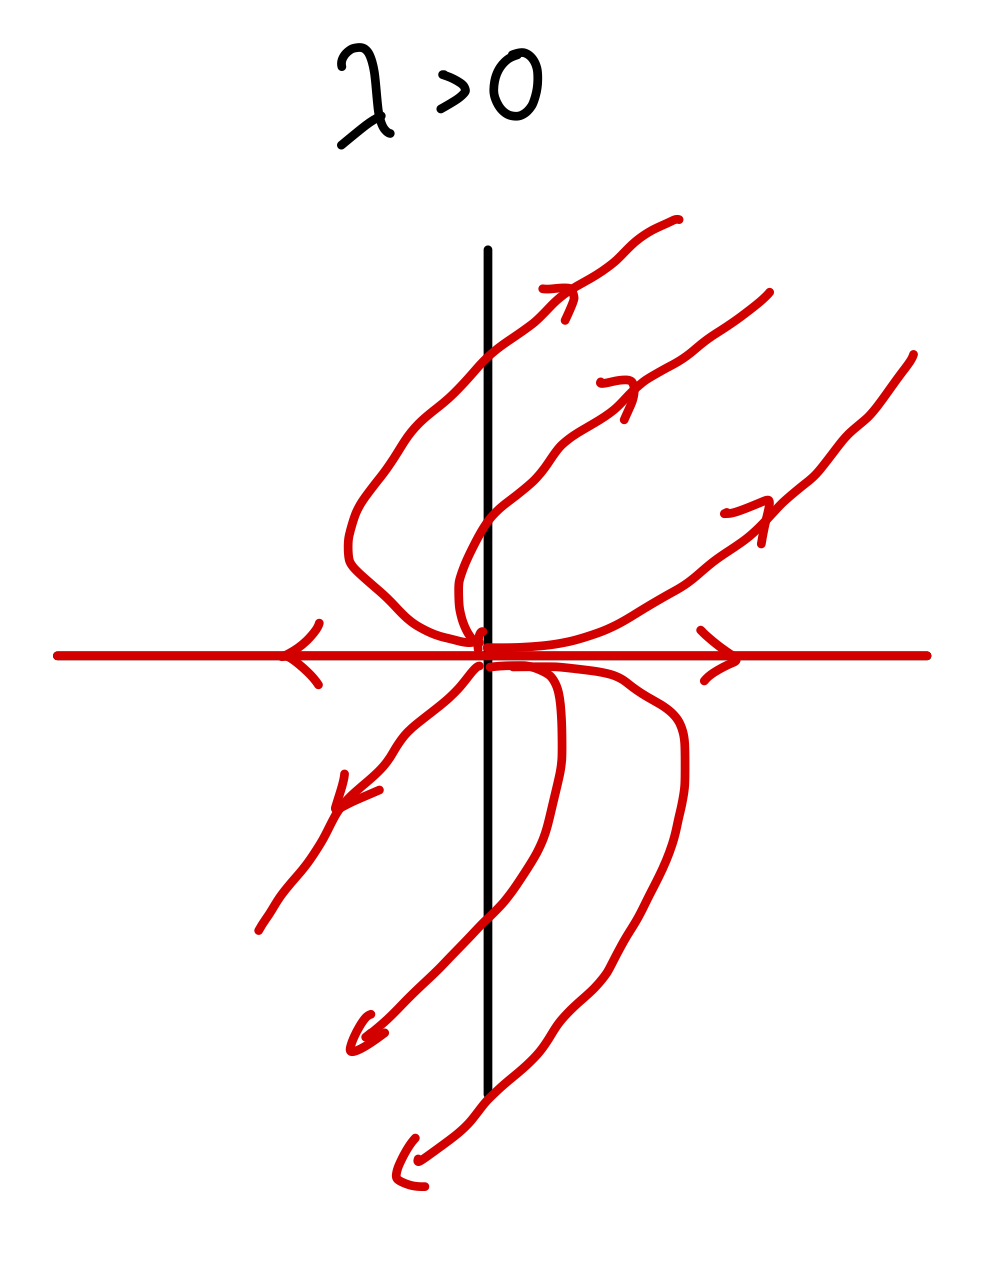
\includegraphics[width=0.2\linewidth]{Bilder/fall2.png}
\end{figure}
\item Fall: $A$ hat zwei komplexe Eigenwerte $\lambda_\pm = a \pm ib$. In einer geeigneten Basis hat $A$ dann die Form
\begin{equation}
A = \mat{a, -b}{b,a} = \mat{a,0}{0,a}+\mat{0,-b}{b,0} = A_1 + A_2.
\end{equation}
Damit gilt
\begin{equation}
\exp(tA) = \exp(tA_1)\exp(tA_2)=\mat{\exp(ta)\cos(b), - \exp(ta) \sin(b)}{\exp(ta) \sin(b), \exp(ta) \cos(b)}.
\end{equation}
\begin{figure}[H]
\label{fig:fall3}
\centering
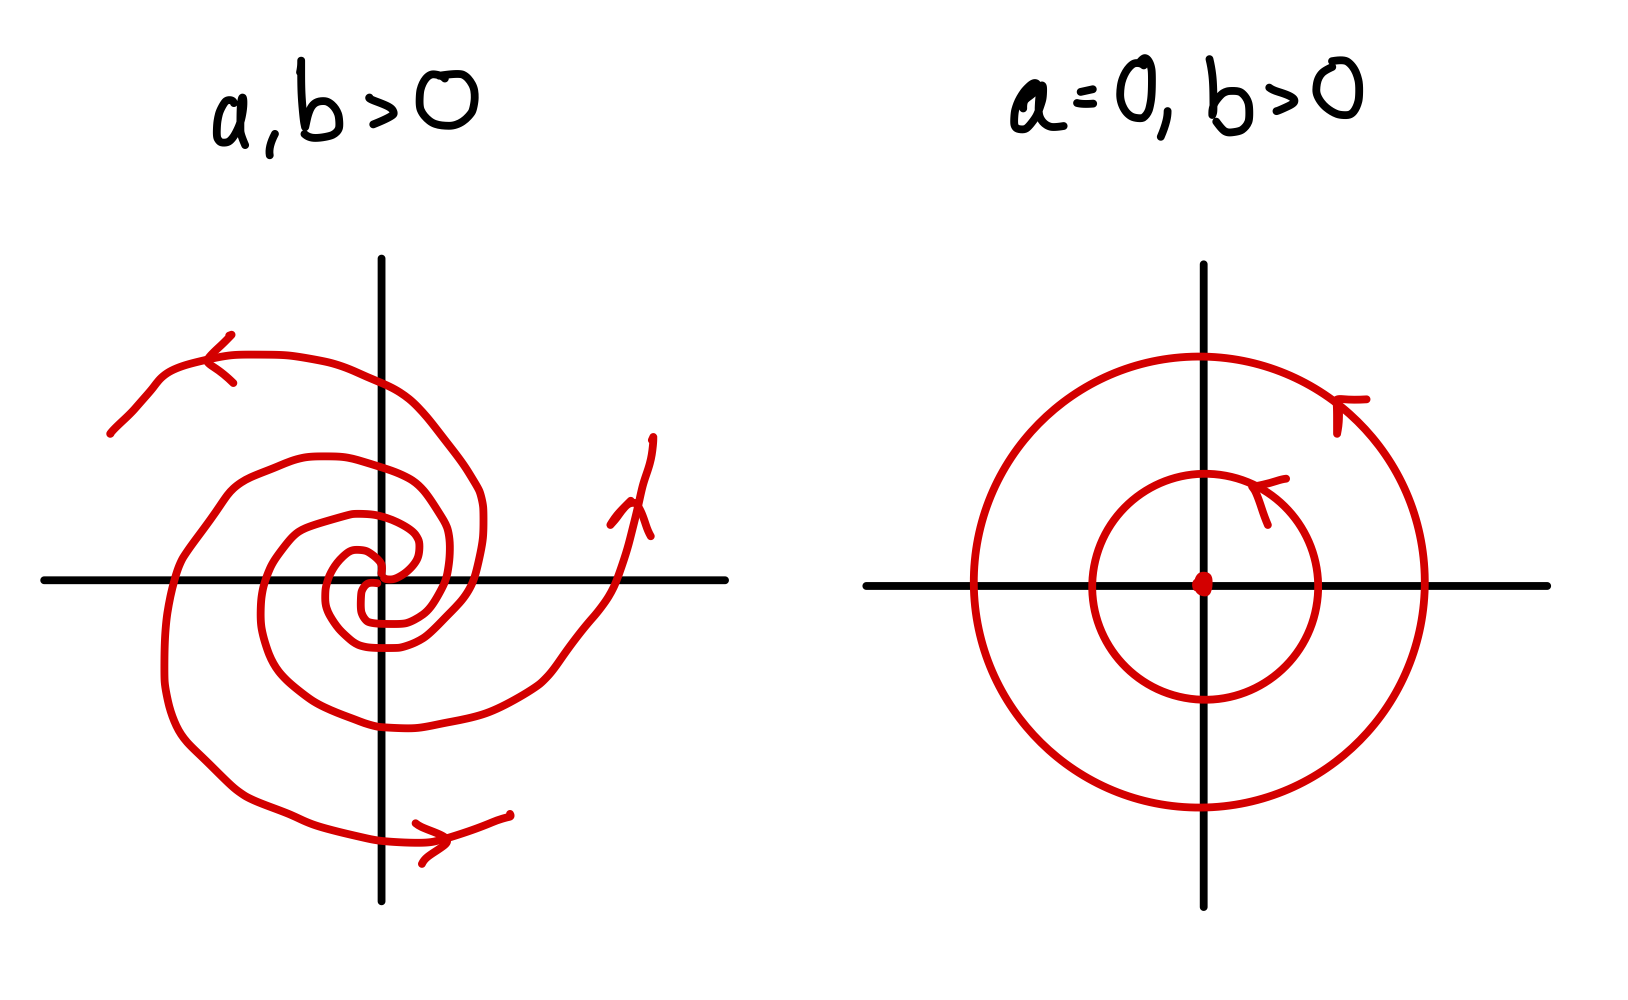
\includegraphics[width=0.3\linewidth]{Bilder/fall3.png}
\end{figure}
\end{enumerate}
\end{bemerkung}
\begin{bemerkung}
Solche linearen DGL sind nützlich für das Studium des qualitativen Verhaltens der Integralkurve eines Vektorfeldes in der Nähe einer isolierten Nullstelle.
\end{bemerkung}
\begin{theorem}{Satz von Grobman-Hartman (Linearisierungssatz)}{grobonanhartman}
Sei $V: \R^n \to \R^n$ ein $\text{C}^1$-Vektorfeld mit $V(0)=0$ und $A := \Ds V_0 \in \text{L}(\R^n, \R^n)$ ohne rein imaginären Eigenwerte.\\
Dann existieren offene Umgebungen $U$ und $U'$ von $0$ und ein \textit{Homöomorphismus} $h: U \to U'$, der Integralkurven von $\dot{x} = V(x)$ in $U$ auf Integralkurven von $\dot{x} = Ax$ in $U'$ abbildet.
\end{theorem}
\begin{beweis}
Geht über den Rahmen der Vorlesung hinaus.
\end{beweis}
